% !TeX document-id = {c68f4be8-c497-43e0-82df-e9ebfbea9577}
% !TeX TXS-program:pdflatex = pdflatex -synctex=1 -interaction=nonstopmode --shell-escape %.tex
% новая команда \RNumb для вывода римских цифр
\documentclass[a4paper,12pt]{article}
\usepackage{amssymb}
\usepackage{amsmath}
\usepackage{amsthm}
\usepackage{caption}
\usepackage{misccorr}
\usepackage[noadjust]{cite}
\usepackage{cmap}
\usepackage[utf8x]{inputenc}
\usepackage[T2A]{fontenc}
\usepackage[english, russian]{babel}
\usepackage{graphics}
\usepackage{graphicx}
\usepackage{textcomp}
\usepackage{verbatim}
\usepackage{makeidx}
\usepackage{geometry}
\usepackage{float}
\usepackage{bm}
\usepackage{esint}
\usepackage{mathtools}
\usepackage{graphicx}
\usepackage{listings}
\usepackage{courier}
\usepackage{multirow}
\usepackage{graphicx}
\usepackage{xcolor}
\usepackage{ucs}


\lstdefinestyle{asm}{
	language={[x86masm]Assembler},
	backgroundcolor=\color{white},
	basicstyle=\footnotesize\ttfamily,
	keywordstyle=\color{blue},
	stringstyle=\color{red},
	commentstyle=\color{gray},
	numbers=left,
	numberstyle=\tiny,
	stepnumber=1,
	numbersep=5pt,
	frame=single,
	tabsize=4,
	captionpos=b,
	breaklines=true
}

\lstset{basicstyle=\fontsize{10}{10}\selectfont,breaklines=true,inputencoding=utf8x,extendedchars=\true}

\lstset{
	literate=
	{а}{{\selectfont\char224}}1
	{б}{{\selectfont\char225}}1
	{в}{{\selectfont\char226}}1
	{г}{{\selectfont\char227}}1
	{д}{{\selectfont\char228}}1
	{е}{{\selectfont\char229}}1
	{ё}{{\"e}}1
	{ж}{{\selectfont\char230}}1
	{з}{{\selectfont\char231}}1
	{и}{{\selectfont\char232}}1
	{й}{{\selectfont\char233}}1
	{к}{{\selectfont\char234}}1
	{л}{{\selectfont\char235}}1
	{м}{{\selectfont\char236}}1
	{н}{{\selectfont\char237}}1
	{о}{{\selectfont\char238}}1
	{п}{{\selectfont\char239}}1
	{р}{{\selectfont\char240}}1
	{с}{{\selectfont\char241}}1
	{т}{{\selectfont\char242}}1
	{у}{{\selectfont\char243}}1
	{ф}{{\selectfont\char244}}1
	{х}{{\selectfont\char245}}1
	{ц}{{\selectfont\char246}}1
	{ч}{{\selectfont\char247}}1
	{ш}{{\selectfont\char248}}1
	{щ}{{\selectfont\char249}}1
	{ъ}{{\selectfont\char250}}1
	{ы}{{\selectfont\char251}}1
	{ь}{{\selectfont\char252}}1
	{э}{{\selectfont\char253}}1
	{ю}{{\selectfont\char254}}1
	{я}{{\selectfont\char255}}1
	{А}{{\selectfont\char192}}1
	{Б}{{\selectfont\char193}}1
	{В}{{\selectfont\char194}}1
	{Г}{{\selectfont\char195}}1
	{Д}{{\selectfont\char196}}1
	{Е}{{\selectfont\char197}}1
	{Ё}{{\"E}}1
	{Ж}{{\selectfont\char198}}1
	{З}{{\selectfont\char199}}1
	{И}{{\selectfont\char200}}1
	{Й}{{\selectfont\char201}}1
	{К}{{\selectfont\char202}}1
	{Л}{{\selectfont\char203}}1
	{М}{{\selectfont\char204}}1
	{Н}{{\selectfont\char205}}1
	{О}{{\selectfont\char206}}1
	{П}{{\selectfont\char207}}1
	{Р}{{\selectfont\char208}}1
	{С}{{\selectfont\char209}}1
	{Т}{{\selectfont\char210}}1
	{У}{{\selectfont\char211}}1
	{Ф}{{\selectfont\char212}}1
	{Х}{{\selectfont\char213}}1
	{Ц}{{\selectfont\char214}}1
	{Ч}{{\selectfont\char215}}1
	{Ш}{{\selectfont\char216}}1
	{Щ}{{\selectfont\char217}}1
	{Ъ}{{\selectfont\char218}}1
	{Ы}{{\selectfont\char219}}1
	{Ь}{{\selectfont\char220}}1
	{Э}{{\selectfont\char221}}1
	{Ю}{{\selectfont\char222}}1
	{Я}{{\selectfont\char223}}1
}

\newcommand{\specchapter}[1]{\chapter*{#1}\addcontentsline{toc}{chapter}{#1}}
\newcommand{\specsection}[1]{\section*{#1}\addcontentsline{toc}{section}{#1}}
\newcommand{\specsubsection}[1]{\subsection*{#1}\addcontentsline{toc}{subsection}{#1}}
\newcommand{\RNumb}[1]{\uppercase\expandafter{\romannumeral #1\relax}}
\newcommand{\jj}{\righthyphenmin=20 \justifying}


% геометрия
\geometry{pdftex, left = 2cm, right = 2cm, top = 2.5cm, bottom = 2.5cm}

\setcounter{tocdepth}{4} % фикс переноса 
\righthyphenmin = 2
\tolerance = 2048

\begin{document}
\thispagestyle{empty}

\noindent \begin{minipage}{0.15\textwidth}
	
\includegraphics[width=\linewidth]{logo}
\end{minipage}
\noindent\begin{minipage}{0.9\textwidth}\centering
	\textbf{Министерство науки и высшего образования Российской Федерации}\\
	\textbf{Федеральное государственное бюджетное образовательное учреждение высшего образования}\\
	\textbf{«Московский государственный технический университет имени Н.Э.~Баумана}\\
	\textbf{(национальный исследовательский университет)»}\\
	\textbf{(МГТУ им. Н.Э.~Баумана)}
\end{minipage}

\noindent\rule{18cm}{3pt}
\newline\newline
\noindent ФАКУЛЬТЕТ $\underline{\text{«Информатика и системы управления»}}$ \newline\newline
\noindent КАФЕДРА $\underline{\text{«Программное обеспечение ЭВМ и информационные технологии»}}$\newline\newline\newline\newline\newline\newline\newline


\begin{center}
	\noindent\begin{minipage}{1.3\textwidth}\centering
	\Large\textbf{   ~~~ Лабораторная работа №1 (часть 1)}\newline
	\textbf{по дисциплине "Операционные системы"}\newline\newline\newline
	\end{minipage}
\end{center}

\noindent\textbf{Тема} $\underline{\text{Дизассемблирование INT 8h}}$\newline\newline
\noindent\textbf{Студент} $\underline{\text{Сапожков А. М.}}$\newline\newline
\noindent\textbf{Группа} $\underline{\text{ИУ7-53Б}}$\newline\newline
\noindent\textbf{Преподаватель} $\underline{\text{Рязанова Н. Ю.}}$\newline

\begin{center}
	\vfill
	Москва~---~\the\year
~г.
\end{center}
\clearpage

% \section{Цель работы}
% Целью первой части лабораторной работы является знакомство со средством дизассемблирования – sourcer и с получением дизассемблерного кода 
% ядра операционной системы Windows на примере обработчика прерывания INT 8h в virtual mode.

\section{Полученный дизассемблированный код}

\subsection{Листинг обработчика прерывания INT 8h} 
\begin{lstlisting}[style={asm}]
; Вызов подпрограммы sub_3:
020A:0746  E8 0070		  	    call	sub_3			    ; (07B9)
; Сохранение значений регистров es, ds, ax, dx:
020A:0749  06				    push	es
020A:074A  1E				    push	ds
020A:074B  50				    push	ax
020A:074C  52				    push	dx
; Загрузка сегментных регистров ds, es: 
; (40h - сегментная часть адреса области данных BIOS)
020A:074D  B8 0040			    mov	ax,40h
020A:0750  8E D8			    mov	ds,ax
020A:0752  33 C0			    xor	ax,ax
020A:0754  8E C0			    mov	es,ax
; Инкремент значений счётчиков таймера:
; 0040:006C, 0040:006E - адреса младшего и старшего слова 
; счётчика прерываний таймера BIOS
020A:0756  FF 06 006C		    inc	word ptr ds:[6Ch]	    ; (0040:006C=9A82h)
020A:075A  75 04			    jnz	loc_2			        ; Jump if not zero
020A:075C  FF 06 006E		    inc	word ptr ds:[6Eh]	    ; (0040:006E=0)
; Сброс счётчиков времени при наступлении нового дня:
; 0040:006E == 18h (24), 0040:006C == B0h (176)
; 18h << 16 + B0h == 86400 * c; 
; c = 1573040 / 86400 = 18.2... - количество срабатываний таймера в секунду
020A:0760			loc_2:
020A:0760  83 3E 006E 18	    cmp	word ptr ds:[6Eh],18h	; (0040:006E=0)
020A:0765  75 15			    jne	loc_3			        ; Jump if not equal
020A:0767  81 3E 006C 00B0	    cmp	word ptr ds:[6Ch],0B0h	; (0040:006C=9A82h)
020A:076D  75 0D			    jne	loc_3			        ; Jump if not equal
020A:076F  A3 006E			    mov	word ptr ds:[6Eh],ax	; (0040:006E=0)
020A:0772  A3 006C			    mov	word ptr ds:[6Ch],ax	; (0040:006C=9A82h)
; Установка флага наращивания даты (начальное значение - 0)
020A:0775  C6 06 0070 01	    mov	byte ptr ds:[70h],1	    ; (0040:0070=0)
; Установка al = 8:
020A:077A  0C 08			    or	al,8
020A:077C			loc_3:
; Сохранение значения регистра ax:
020A:077C  50				    push	ax
; Декремент значения счётчика времени до отключения моторчика дисковода:
; (0040:0040 - адрес счётчика времени в области данных накопителя FDD)
020A:077D  FE 0E 0040		    dec	byte ptr ds:[40h]	    ; (0040:0040=39h)
020A:0781  75 0B			    jnz	loc_4			        ; Jump if not zero
; Установка флагов, отвечающих за отключение моторчикка дисковода:
020A:0783  80 26 003F F0	    and	byte ptr ds:[3Fh],0F0h	; (0040:003F=0)
; Отправка команды отключения моторчика дисковода:
020A:0788  B0 0C			    mov	al,0Ch
020A:078A  BA 03F2			    mov	dx,3F2h
020A:078D  EE				    out	dx,al			        ; port 3F2h, dsk0 contrl output
020A:078E			loc_4:
; Восстановление значения регистра ax:
020A:078E  58				    pop	ax
; Проверка второго бита (Parity Flag - флаг чётности):
; 0040:0314h - адрес области данных BIOS, содержащей копию флагов
020A:078F  F7 06 0314 0004	    test	word ptr ds:[314h],4	; (0040:0314=3200h)
020A:0795  75 0C			    jnz	loc_5			        ; Jump if not zero
; Сохранение младшего байта регистра FLAGS в AH:
020A:0797  9F				    lahf				        ; Load ah from flags
; Обмен значений регистров ah и al: 
; Теперь младший байт регистра FLAGS находится в младшем байте регистра ax
020A:0798  86 E0			    xchg	ah,al
; Сохранение регистра ax:
020A:079A  50				    push	ax
; Косвенный вызов пользовательского прерывания по адресу в таблице векторов прерываний:
; В этом случае не произойдёт push регистра FLAGS, на его месте будет AX, 
; который восстановится в регистр FLAGS после выхода из обработчика прерывания
020A:079B  26: FF 1E 0070	    call	dword ptr es:[70h]	; (0000:0070=6ADh)
020A:07A0  EB 03			    jmp	short loc_6		        ; (07A5)
020A:07A2  90				    nop
; Вызов пользовательского прерывания через int 1Ch:
020A:07A3			loc_5:
020A:07A3  CD 1C			    int	1Ch			            ; Timer break (call each 18.2ms)
020A:07A5			loc_6:
; Вызов подпрограммы sub_3, чтобы запретить вызов int 8h:
020A:07A5  E8 0011			    call	sub_3			    ; (07B9)
; Сброс контроллера прерываний (отправка команды End Of Interrupt):
; Разрешение обработки всех прерываний
020A:07A8  B0 20			    mov	al,20h		; ' '
020A:07AA  E6 20			    out	20h,al		; port 20h, 8259-1 int command
                                                ; al = 20h, end of interrupt
; Восстановление значений регистров es, ds, ax, dx:
020A:07AC  5A				    pop	dx
020A:07AD  58				    pop	ax
020A:07AE  1F				    pop	ds
020A:07AF  07				    pop	es
020A:07B0  E9 FE99			    jmp	$-164h 				    ; 020A:07B0h - 164h = 020A:064Ch
; ...
; Возврат из прерывания
020A:06AC  CF					iret						; Interrupt return
\end{lstlisting}

% \clearpage
\subsection{Листинг процедуры sub\_3}

\begin{lstlisting}[style={asm}]
020A:07B9		sub_3		proc	near
; Сохранение значений регистров ds, ax:
020A:07B9  1E				push	ds
020A:07BA  50				push	ax
; Загрузка сегментного регистра ds:
020A:07BB  B8 0040			mov	ax,40h
020A:07BE  8E D8			mov	ds,ax
; Запись младшего байта регистра FLAGS в AH:
020A:07C0  9F				lahf				                    ; Load ah from flags
; Проверка DF и старшего бита IOPL по адресу 0040:0314h:
020A:07C1  F7 06 0314 2400	test	word ptr ds:[314h],2400h	    ; (0040:0314=3200h)
020A:07C7  75 0C			jnz	loc_8			                    ; Jump if not zero
; Установка 9 бита в 0 - сброс IF (запрет прерываний):
020A:07C9  F0> 81 26 0314 FDFF	lock and word ptr ds:[314h],0FDFFh	; (0040:0314=3200h)
020A:07D0		loc_7:
; Запись регистра AH в младший байт FLAGS:
020A:07D0  9E				sahf				                    ; Store ah into flags
; Восстановление значений регистров ds, ax:
020A:07D1  58				pop	ax
020A:07D2  1F				pop	ds
020A:07D3  EB 03			jmp	short loc_9		                    ; (07D8)
020A:07D5		loc_8:
; Сброс флага IF:
020A:07D5  FA				cli				                        ; Disable interrupts
020A:07D6  EB F8			jmp	short loc_7		                    ; (07D0)
020A:07D8		loc_9:
; Возврат из подпрограммы:
020A:07D8  C3				retn
				sub_3	    endp
\end{lstlisting}
\clearpage

\section{Схема алгоритмов}

\subsection{Схема алгоритма обработчика INT8h}
""\newline

\begin{flushright}
	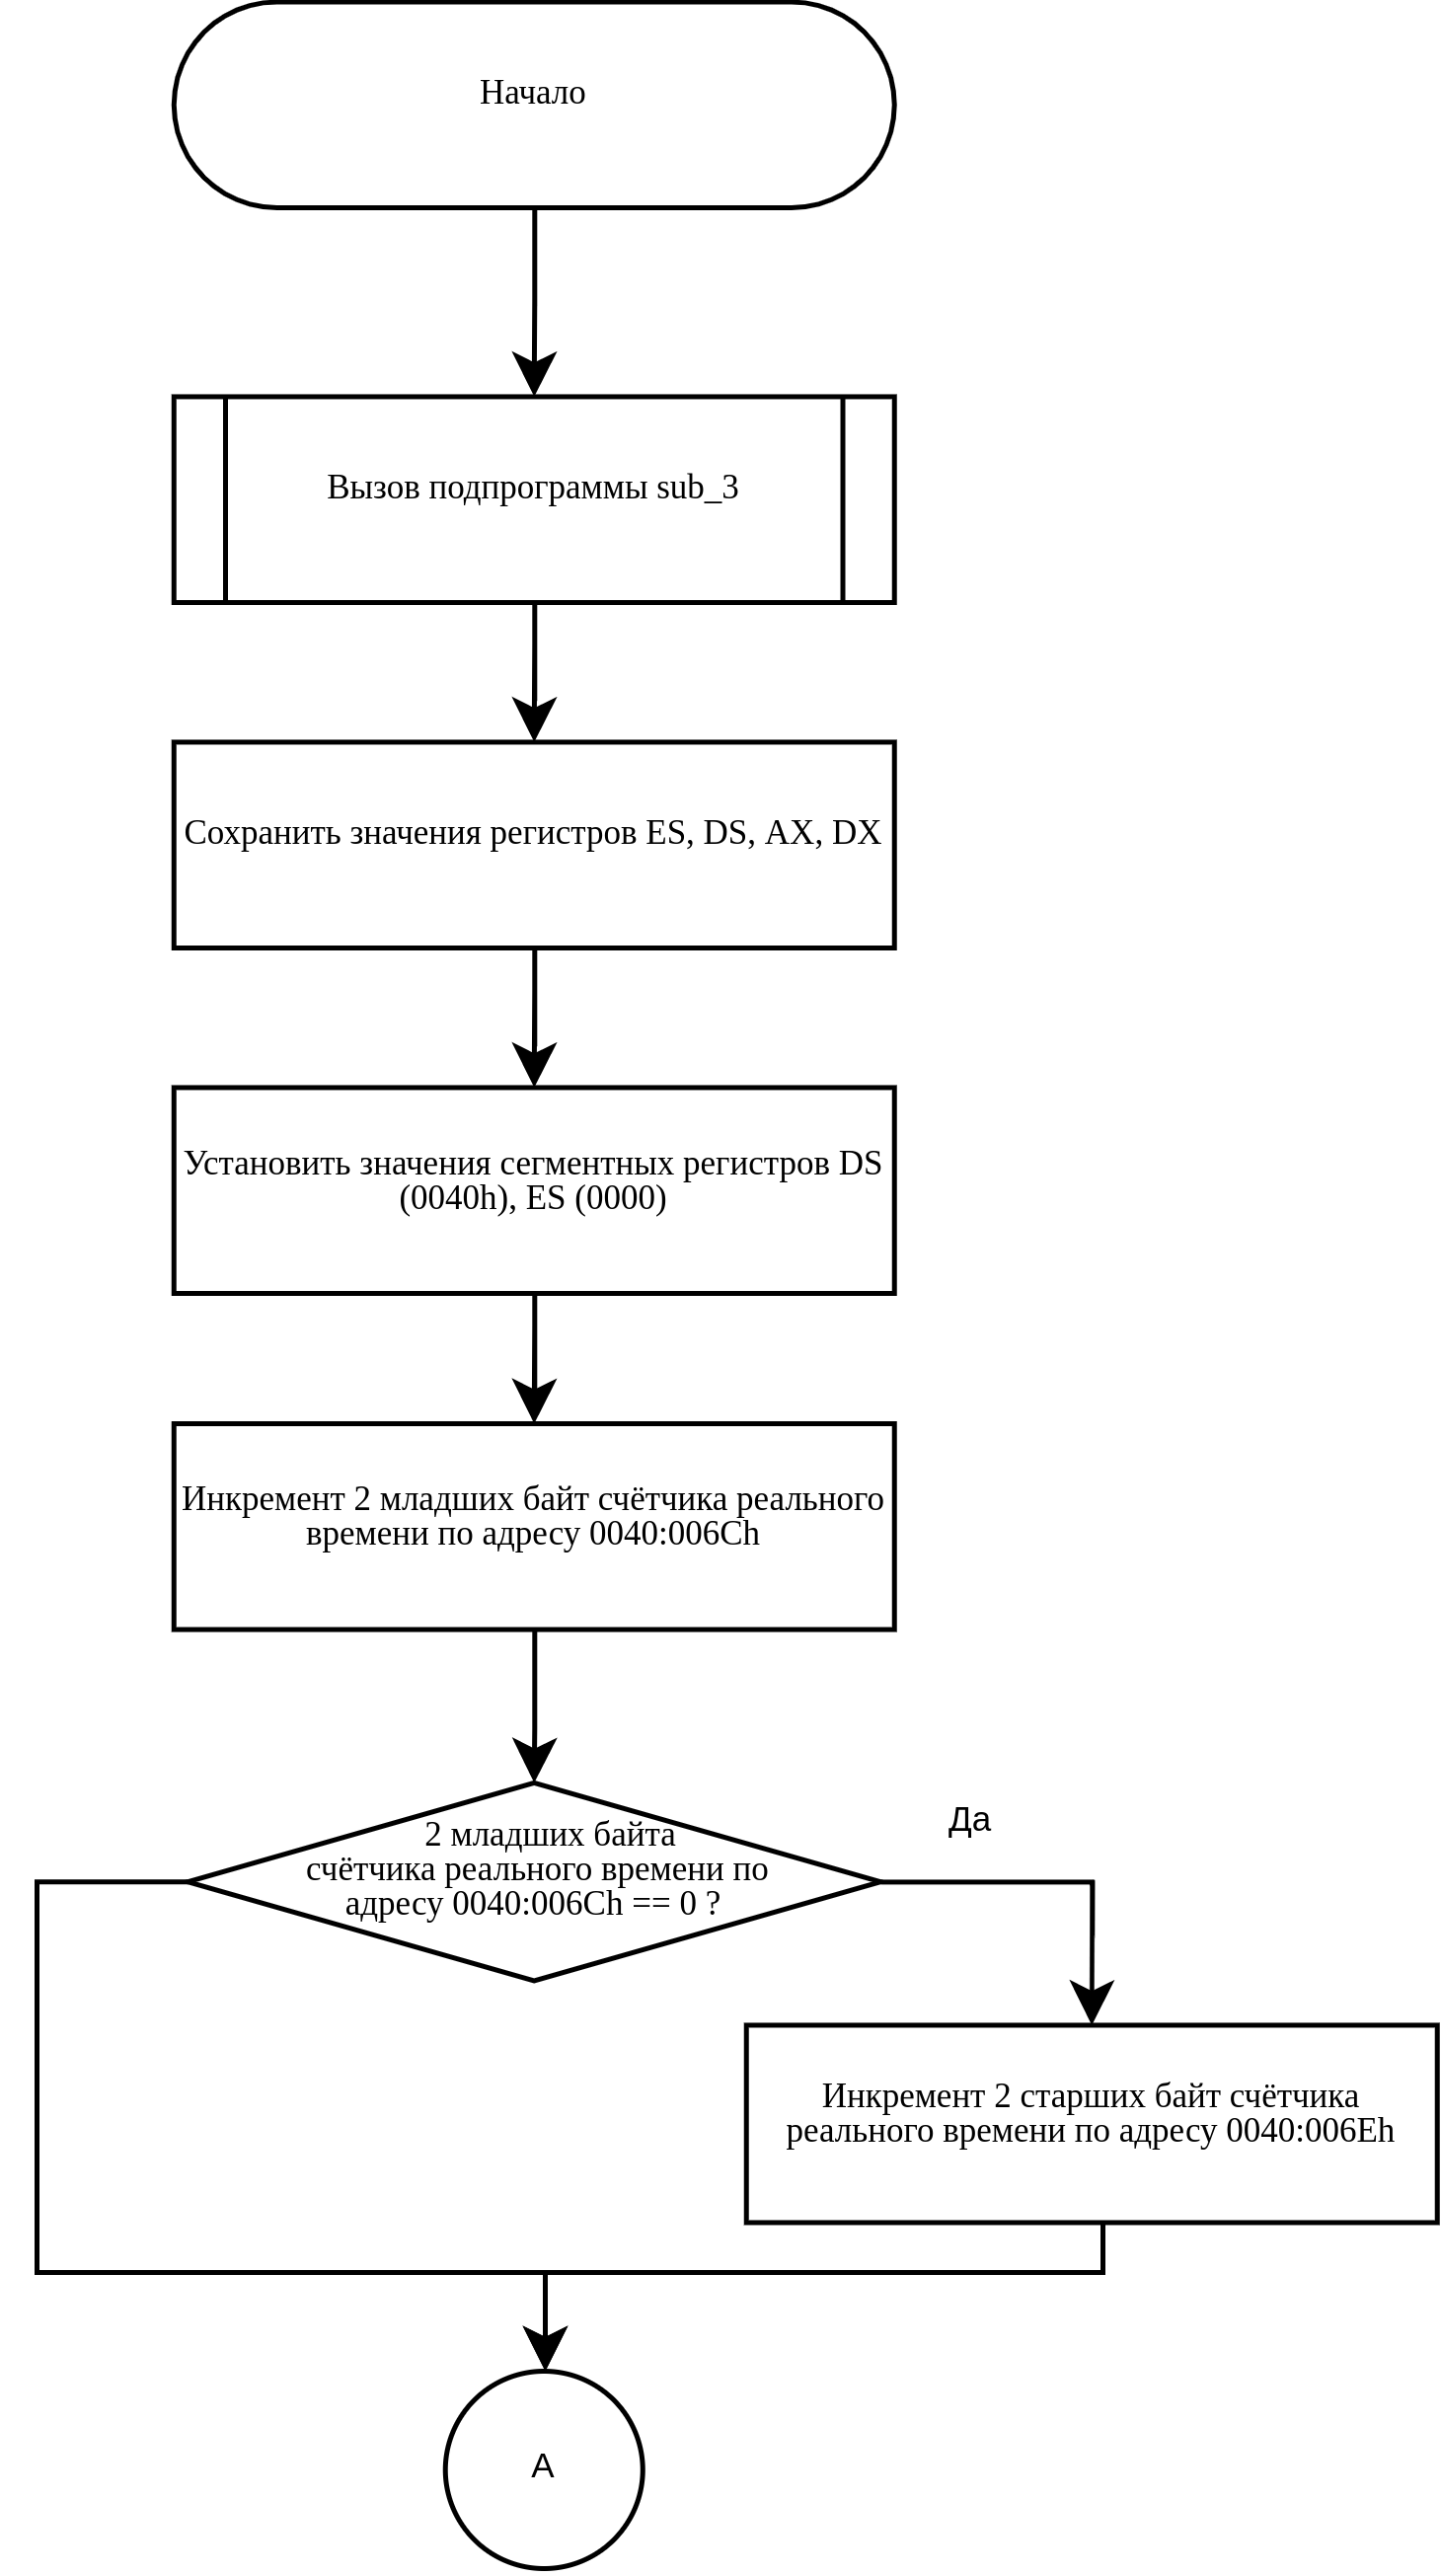
\includegraphics[height=0.875\textheight]{flowchart/int_8h_1.png}
	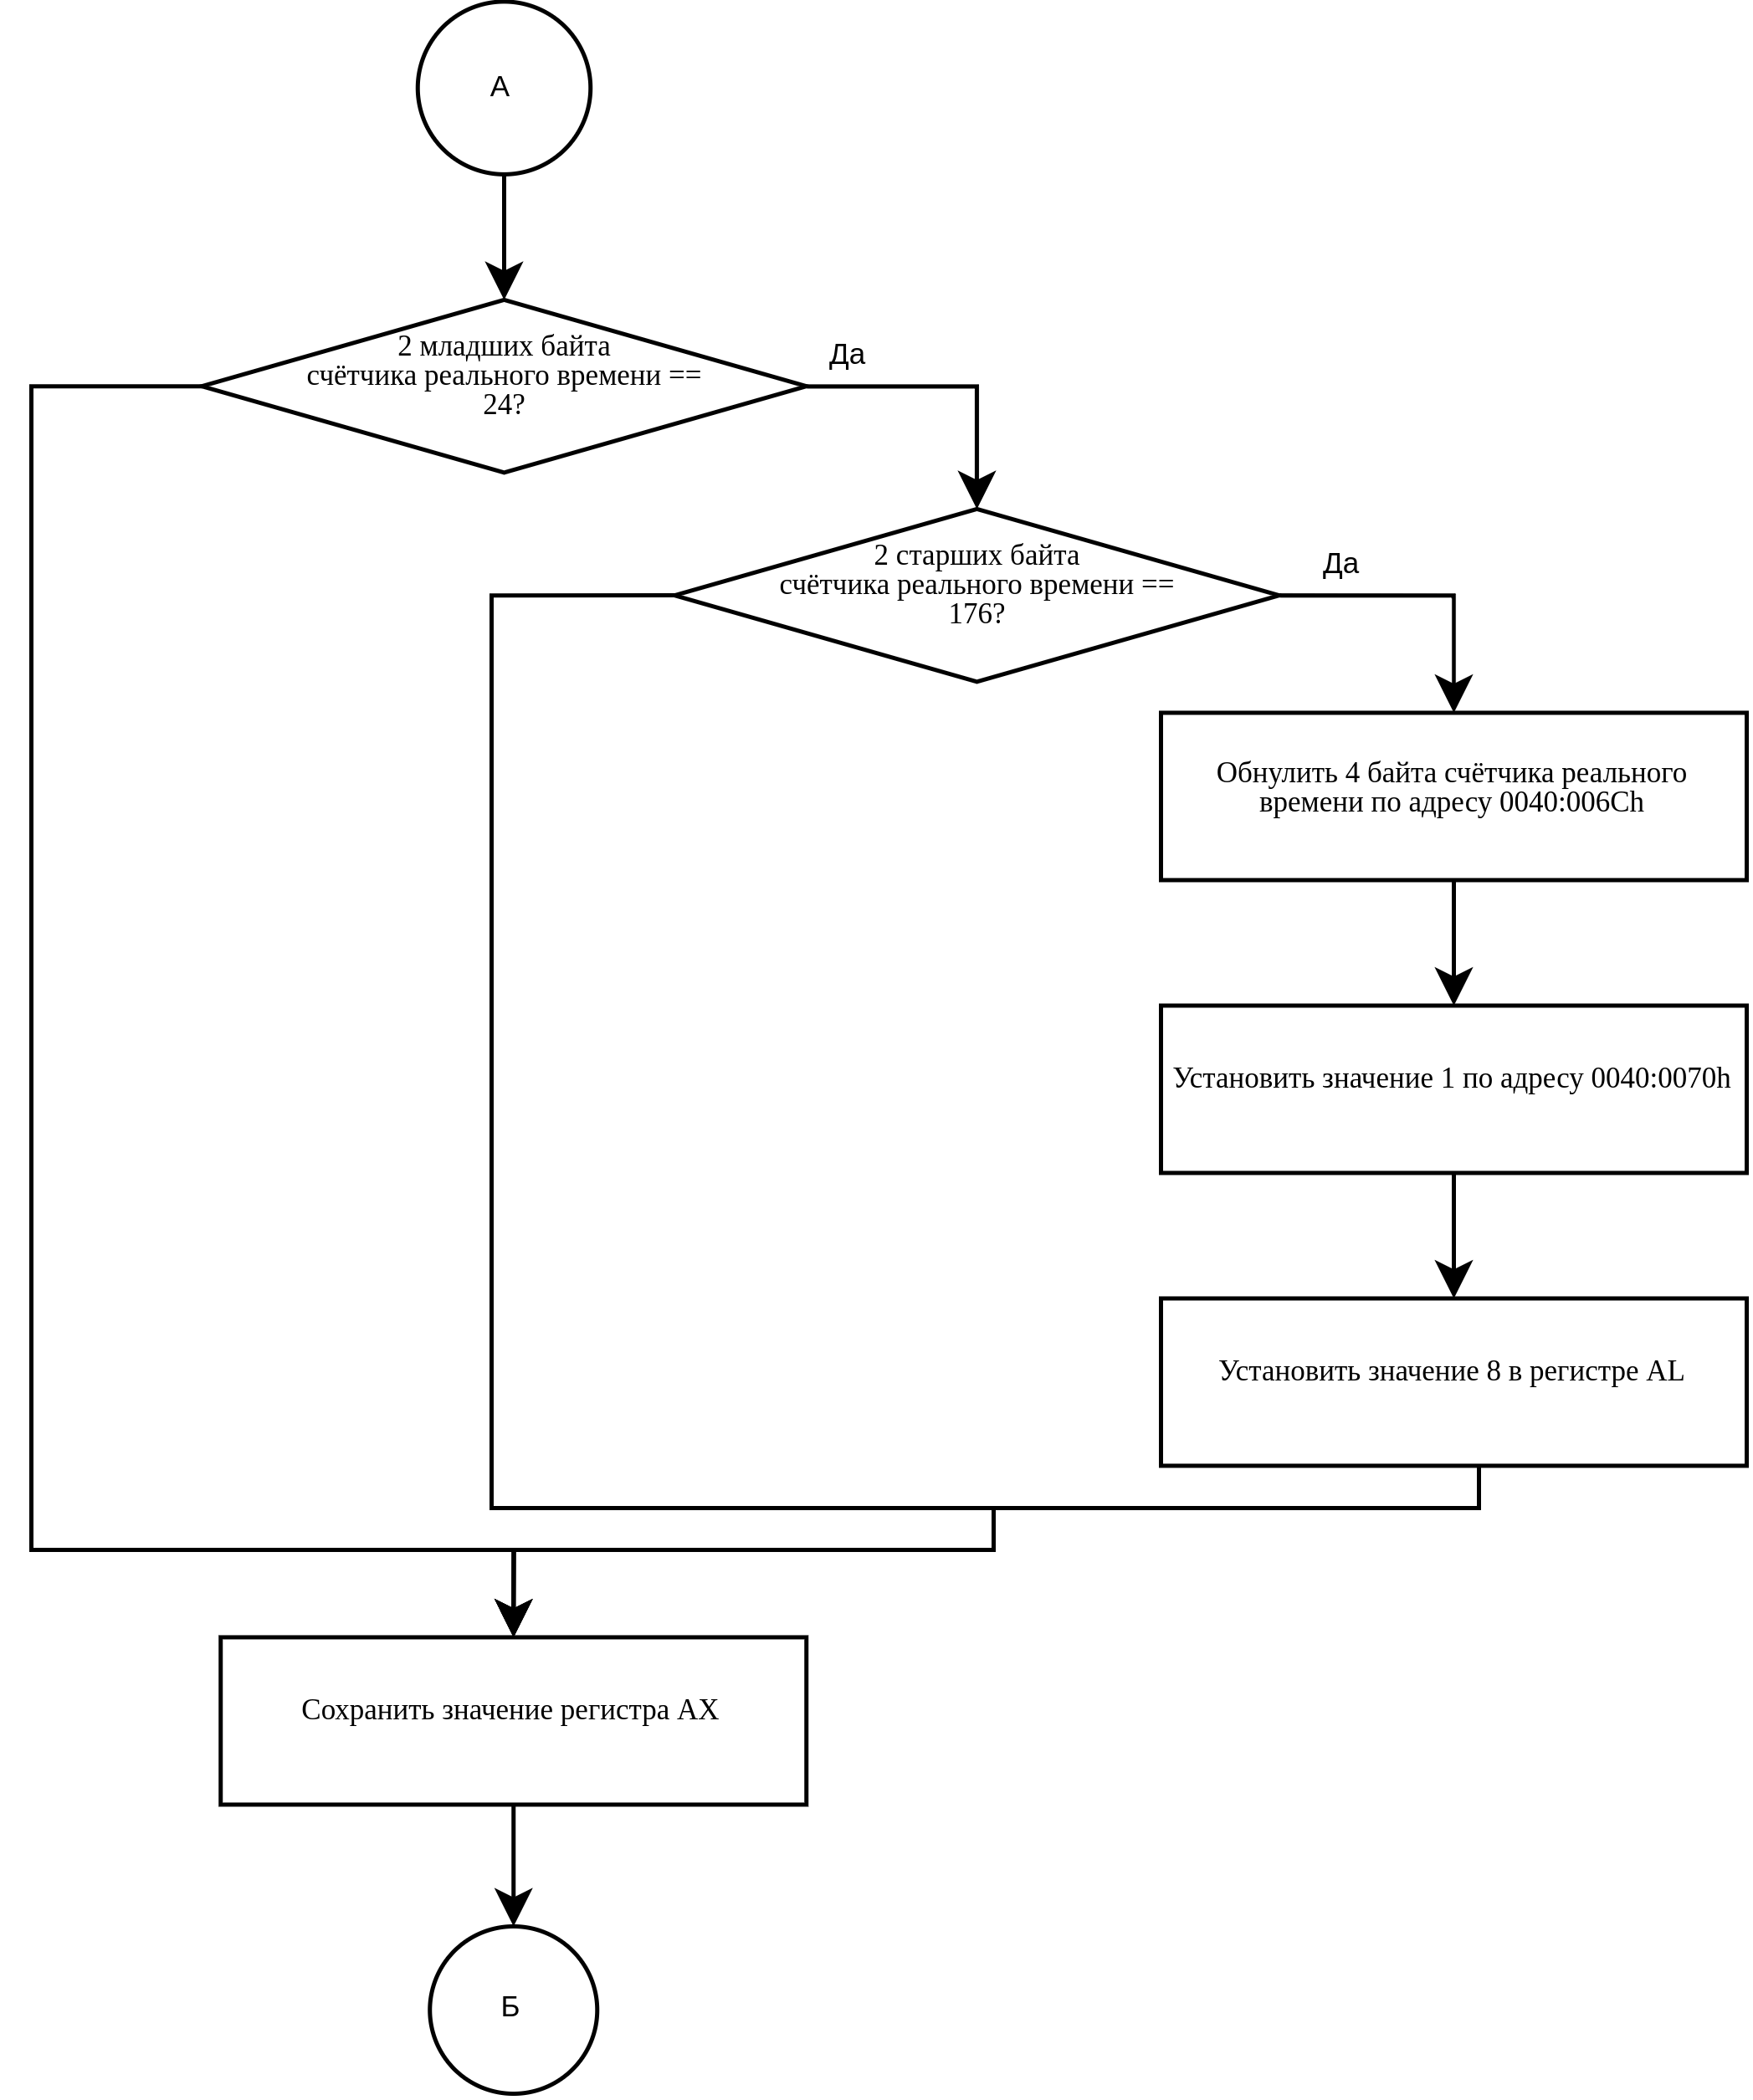
\includegraphics[height=0.9\textheight]{flowchart/int_8h_2.png}
	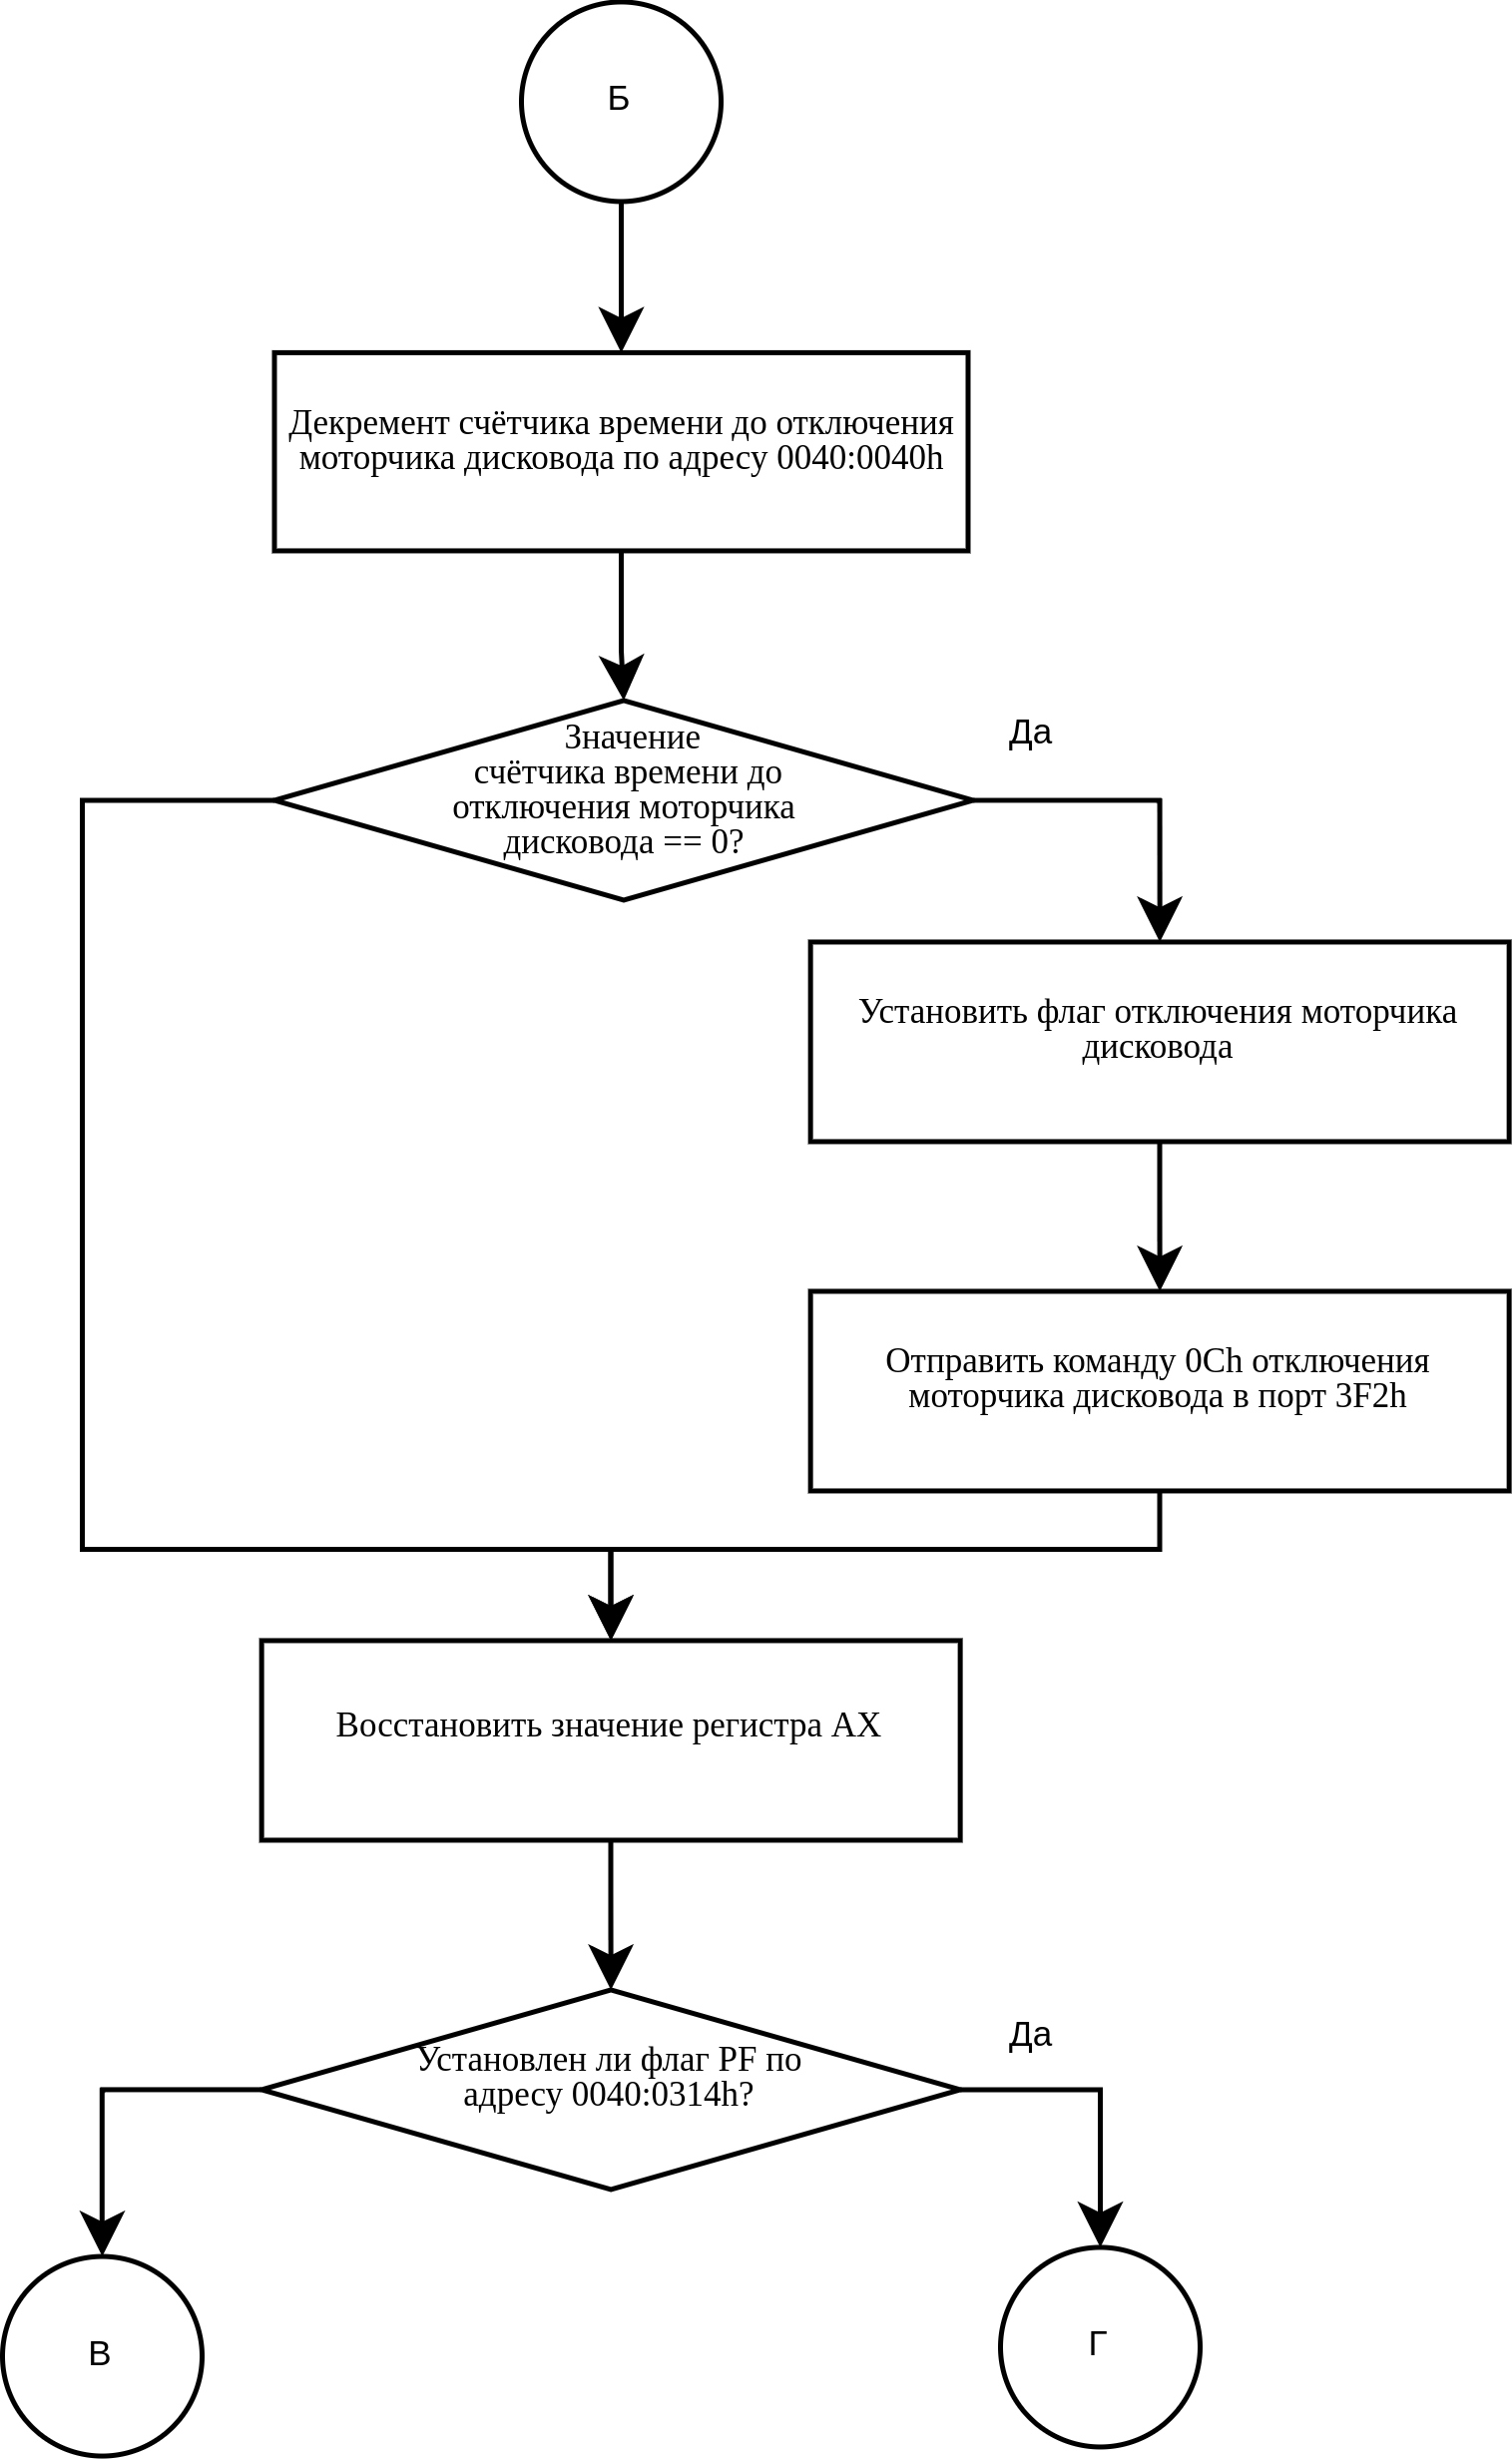
\includegraphics[height=\textheight]{flowchart/int_8h_3.png}
	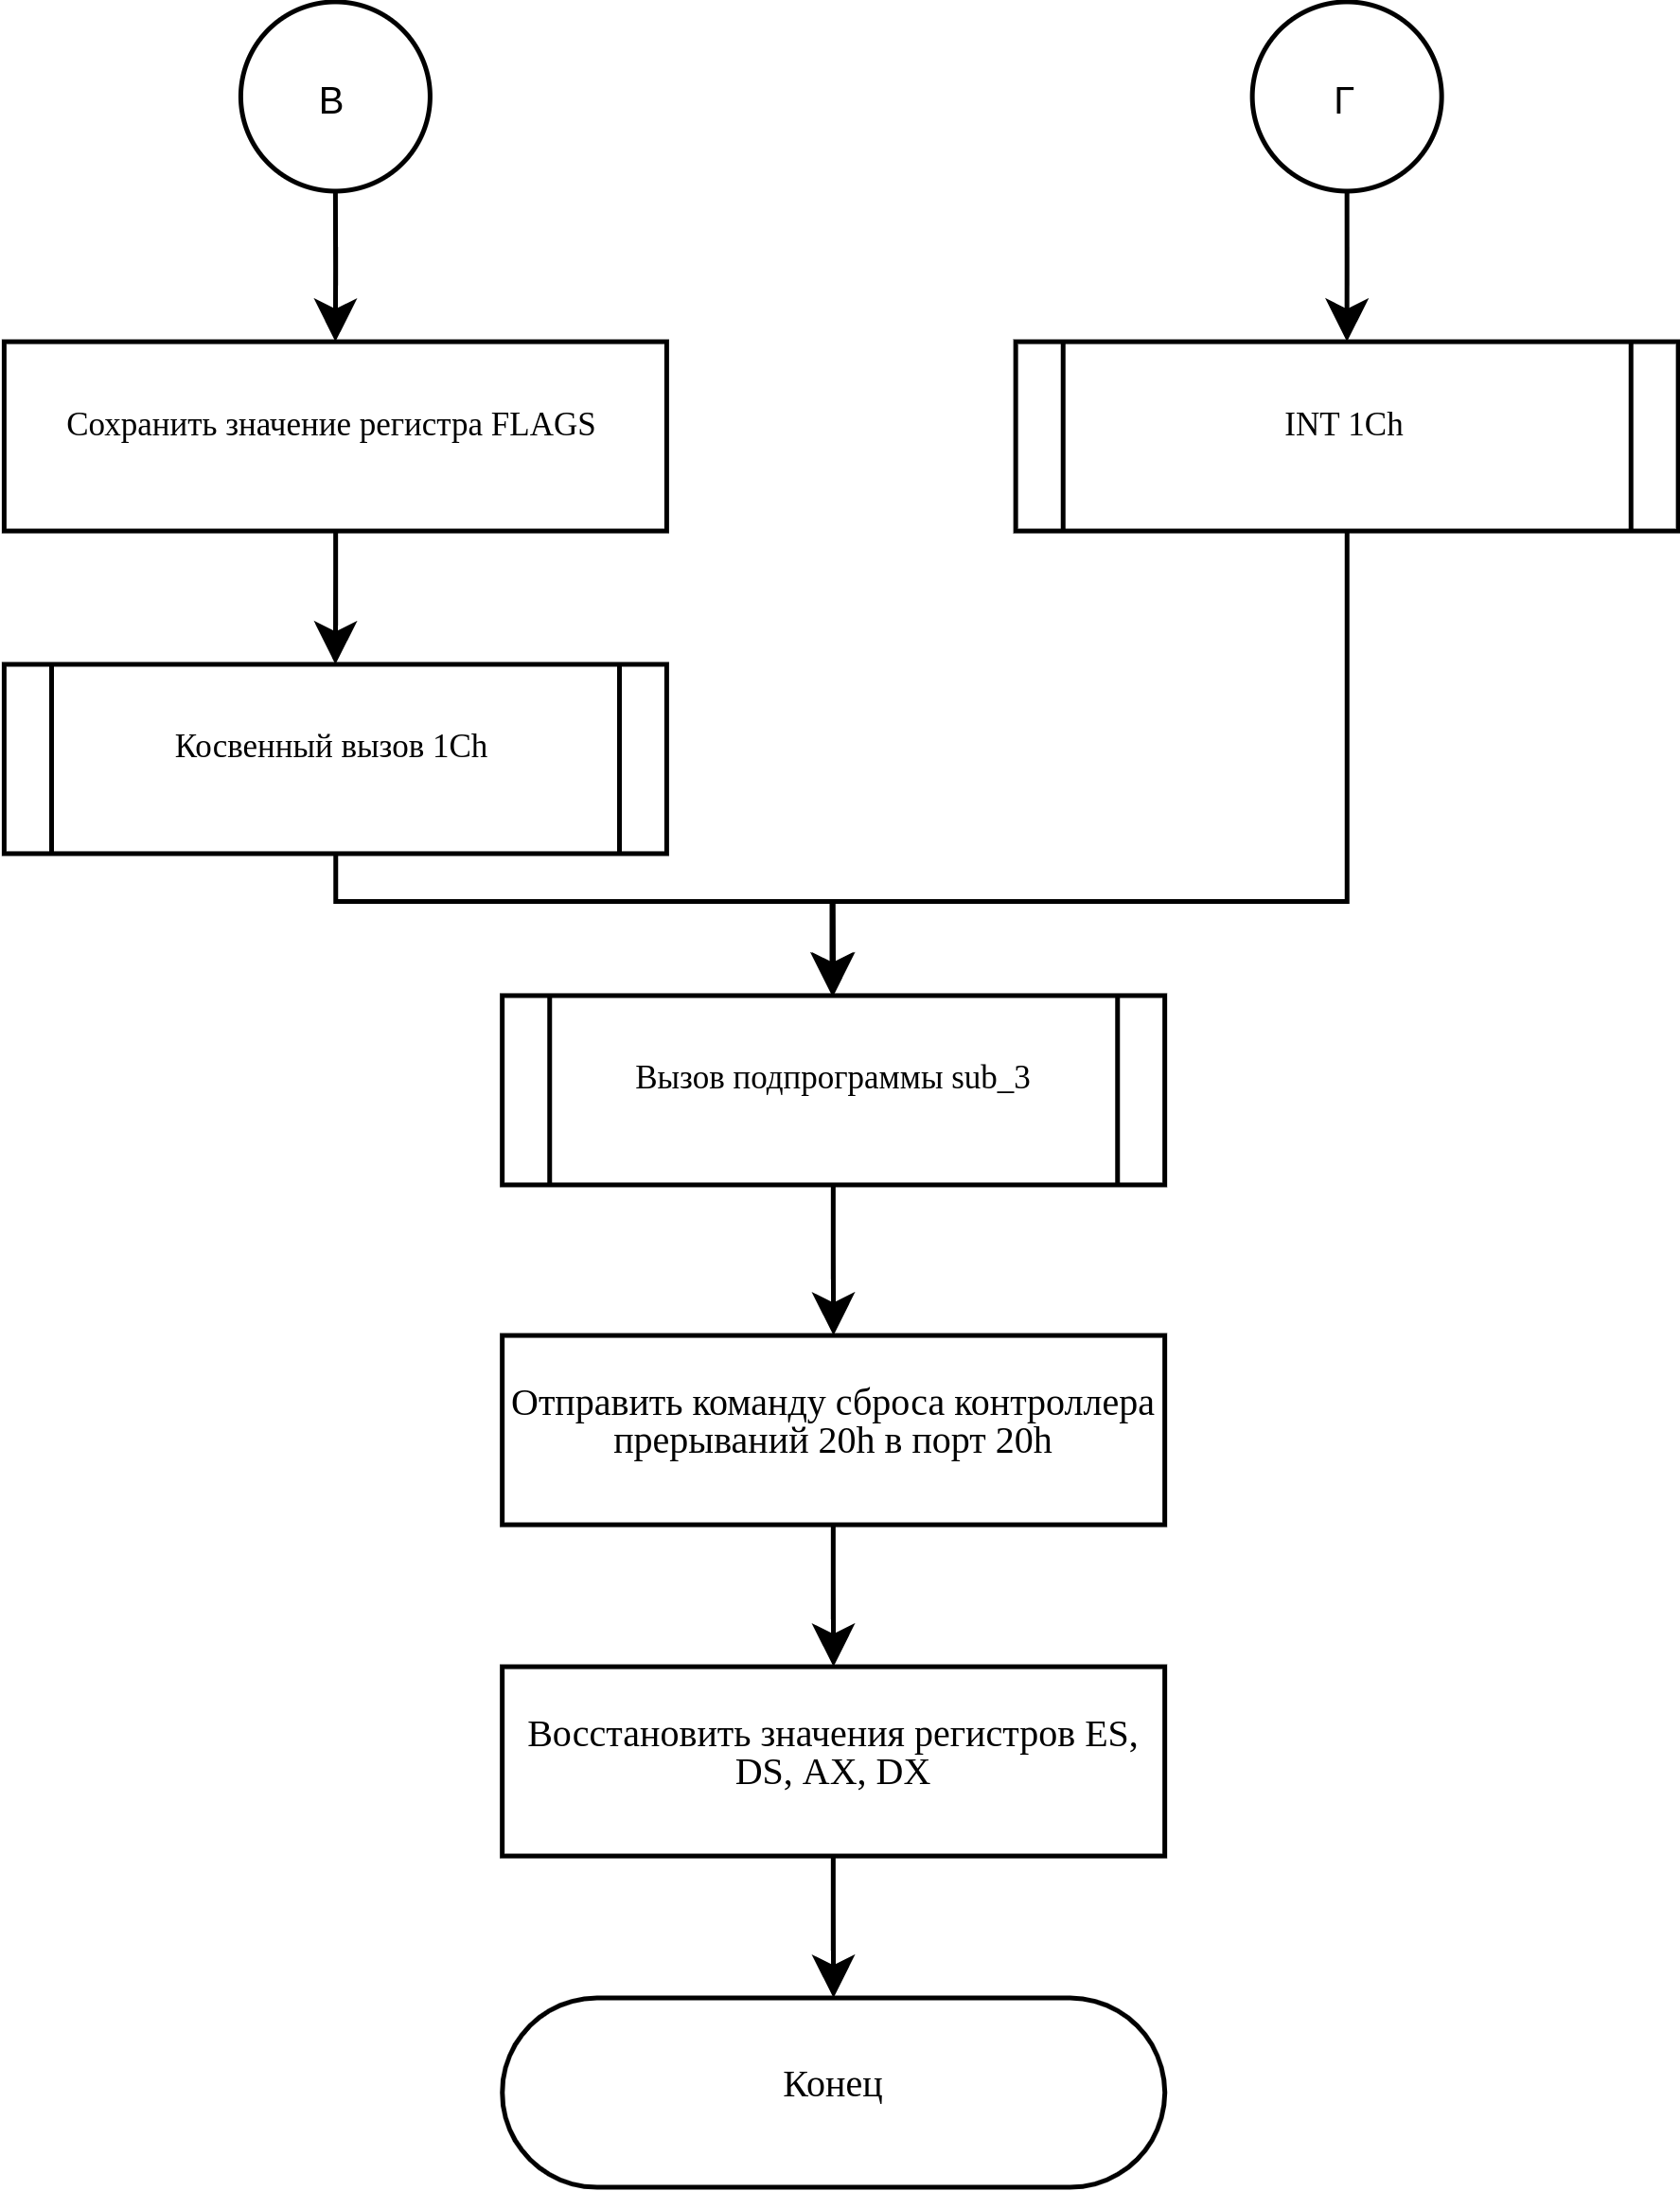
\includegraphics[height=0.95\textheight]{flowchart/int_8h_4.png}
\end{flushright}

% \clearpage
\subsection{Схема алгоритма процедуры sub\_3}

\begin{center}
	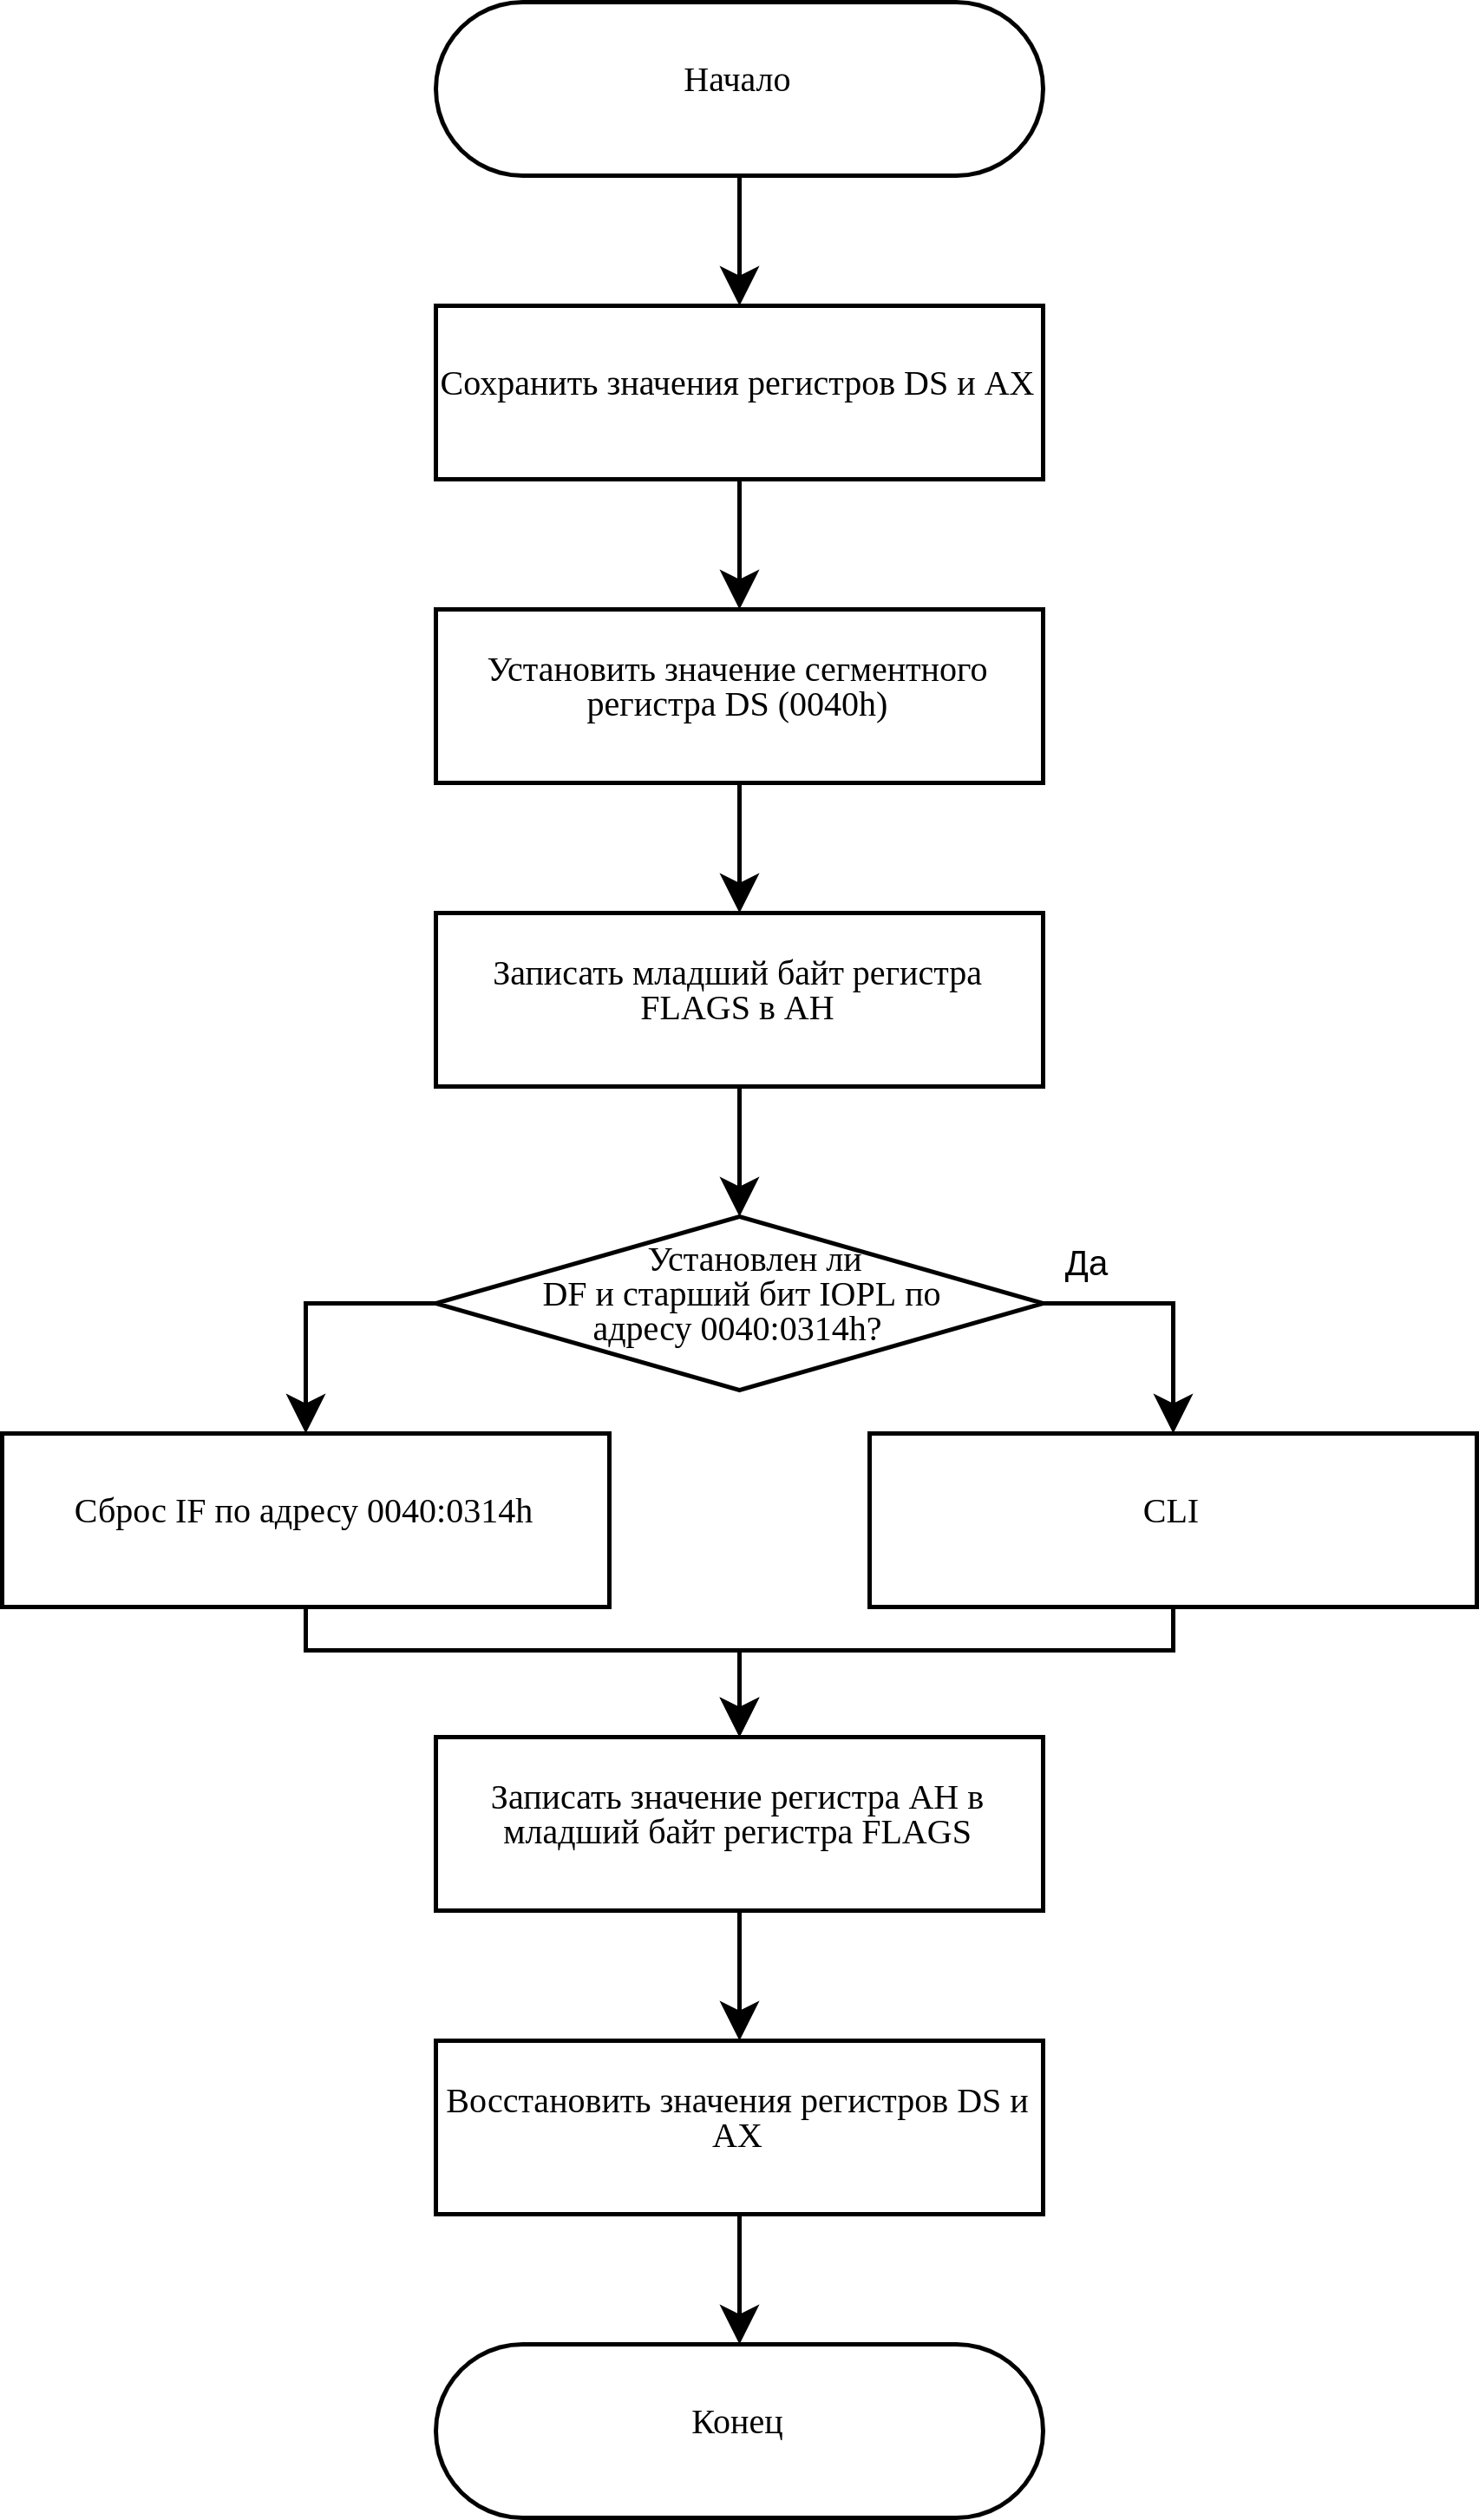
\includegraphics[height=0.98\textheight]{flowchart/subroutine.png}
\end{center}

% \section{Заключение}
% Выполнив данную лабораторную работу, я научился получать адреса и листинги обработчиков прерываний с помощью утилиты debug и дизассемблера 
% soucer соответственно. Также я изучил алгоритм работы обработчика прерывания INT 8h. Это прерывание отвечает за изменение системного 
% времени, управление контроллером дисковода и вызов пользовательского прерывания INT 1Ch.

\end{document}
